%versi 2 (8-10-2016)
\chapter{Landasan Teori}
\label{chap:teori}

\section{Penjadwalan Secara Umum}
\label{sec:penjadwalan} 
 Secara umum penjadwalan menurut Baker (1974) ~\cite{barker:74:introduction} didefinisikan sebagai proses pengalokasian sumber-sumber dalam jangka waktu tertentu untuk melakukan sekumpulan pekerjaan. Definisi ini mengandung dua arti yang berbeda, yaitu :
 \begin{enumerate}
 	\item Penjadwalan merupakan fungsi pengambilan keputusan, yaitu menentukan jadwal. 
 	\item Penjadwalan merupakan suatu teori, yaitu sekumpulan prinsip-prinsip dasar, model-model, teknik-teknik, dan kesimpulan-kesimpulan logis dalam proses pengambilan keputusan yang memberikan dalam fungsi penjadwalan (nilai konseptual).
 \end{enumerate}
	Tujuan penjadwalan secara umum menurut Baker (1974) ~\cite{berg:08:compgeom} adalah :
\begin{enumerate}
	\item Meningkatkan produktivitas mesin, yaitu dengan mengurangi waktu menganggur mesin.
	\item Mengurangi terhadap persediaan barang setengah jadi, dengan mengurangi rata-rata pekerjaan yang menunggu dalam antrian karena mesin sibuk oleh pekerjaan lain.
	\item Mengurangi keterlambatan (tardiness). Dalam banyak hal, beberapa atau semua pekerjaan mempunyai batas waktu penyelesaian (duedate). Apabila suatu pekerjaan melewati batas waktu tersebut, maka akan dikenai pinalti. Keterlambatan dapat diperkecil dengan mengurangi maksimal tardiness atau mengurangi pekerjaan yang terlambat (number of  tardy job).
\end{enumerate}
	Menurut Baker ~\cite{baker:1974:introduction} masalah penjadwalan muncul karena keterbatasan :
	\begin{itemize}
		\item Waktu
		\item Tenaga Kerja
		\item Jumlah Mesin
		\item Sifat dan syarat pekerja.
	\end{itemize}

\subsection{Istilah-Istilah dalam Penjadwalan}
Bedworth ~\cite{Bedworth:1999:IPC:554704} menyebutkan beberapa istilah dalam penjadwalan yang perlu dijelaskan adalah sebagai berikut:
 \begin{itemize}
 	\item Waktu Pemrosesan ({\it Processing Time }) \\
 	Lamanya waktu yang dibutuhkan untuk menyelesaikan satu aktivitas pekerjaan.
 	\item Makespan \\
 	Keseluruhan waktu yang dibutuhkan untuk menyelesaikan aktivitas pekerjaan.
 	\item Waktu Aliran (Flow Time) \\
 	Rentang waktu antara satu pekerjaan dapat dimulai sampai saat dimana pekerjaan tersebut selesai dikerjakan. Sehingga waktu aliran sama dengan waktu pemrosesan ditambah dengan waktu menunggu sebelum diproses.
	\item Waktu Penyelesaian (Completion Time)\\
	Waktu dimana tugas terakhir dari satu pekerjaan tertentu selesai dikerjakan.
	\item Batas Waktu (Due Time)\\
	Batas waktu penyelesaian untuk suatu pekerjaan (order) dan jika suatu pekerjaan (order)
	melewati batas waktu tersebut akan dikenakan denda (penalty)
	\item Tardiness \\
	Merupakan keterlambatan penyelesaian suatu job  terhadap batas waktu penyelesaian (due time) job tersebut.
 	
 \end{itemize}

\subsection{Klasifikasi Masalah Penjadwalan}

	Permasalahan penjadwalan dapat dilihat dari : 
\begin{enumerate}
	\item Mesin :
	\begin{itemize}
		\item Mesin Tunggal
		\item Mesin ganda (2 mesin)
		\item M mesin
	\end{itemize}
	\item Aliran proses
	\begin{itemize}
		\item {\it Job Shop}
		\item {\it Flow Shop}
	\end{itemize}
	\item Pola Kedatangan
	\begin{itemize}
		\item Statis
		\item Dinamis
	\end{itemize}

\end{enumerate}





\section{Penjadwalan Flow Shop}
\label{sec:Flowshop}

Seperti yang telah disebutkan di atas. Penjadwalan berdasarkan aliran proses terdiri atas dua penjadwalan yaitu :
\begin{enumerate}
	\item {\it Job Shop}\\
	Setiap proses pekerjaan yang dikerjakan tidak memiliki lintasan operasi yang tetap, artinya
	setiap job yang datang memiliki proses operasi yang berbeda dan dapat mengalami pengulangan
	lintasan. Gambar~\ref{fig:JobShop} merupakan gambaran dari pola kerja job shop. Pada gambar tersebut dijelaskan 
	bahwa P1 akan jalan melalui mesin 1 ke mesin 2. Lalu pada P3 di jelaskan job dimulai dari mesin ke 4 lalu ke mesin 3, 
	maka dapat disimpulkan setiap job memiliki proses operasi yang berbeda.
	\begin{figure}[H]
		\centering  
		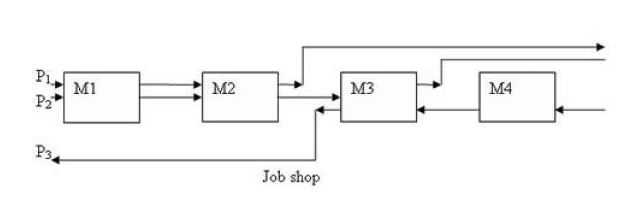
\includegraphics[scale=0.5]{JobShop}  
		\caption[Job Shop]{Job Shop} 
		\label{fig:JobShop} 
	\end{figure}
	
			
	\item {\ Flow shop}\\
	Setiap pekerjaan yang akan diproses memiliki lintasan produksi yang searah, dan setiap operasi
	yang dilalui oleh setiap job memiliki urutan proses yang sama tanpa mengalami pengulangan
	lintasan (semua job hanya diproses sekali pada tiap mesin). Gambar~\ref{fig:FlowShop} merupakan
	gambaran dari pola kerja flow shop.
	\begin{figure}[H]
		\centering  
		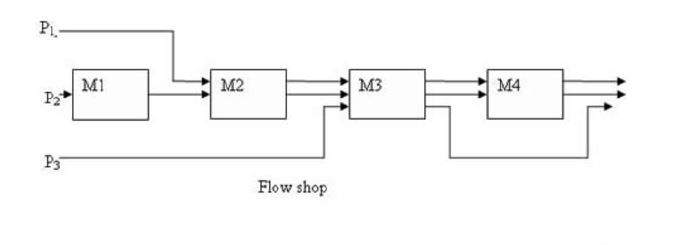
\includegraphics[scale=0.5]{FlowShop}  
		\caption[Flow Shop]{Flow Shop} 
		\label{fig:FlowShop} 
	\end{figure}
	
\end{enumerate}

\subsection{Definisi Secara Umum}
Permasalahan flow shop scheduling adalah bagaimana menentukan urutan pengerjaan untuk sejumlah
n job dengan menggunakan sejumlah m mesin dalam urutan proses yang sama dan setiap job
melewati setiap mesin dalam satu waktu tertentu. Masing-masing job memiliki lama pengerjaan
yang berbeda. Dalam pemrosesan, setiap job membutuhkan sebanyak m operasi (setiap mesin satu
operasi). Setiap job tidak dapat saling mendahului dan setiap mesin tidak akan diam saat job siap
diproses.
Tujuan utama dari flow shop scheduling adalah menentukan makespan minimum untuk mengerjakan
n job dengan menggunakan m mesin. Nilai makespan dapat berubah-ubah berdasarkan
urutan pengerjaan job yang dilakukan, oleh karena itu urutan pengerjaan akan sangat berpengaruh terhadap nilai makespan.
Pada skripsi ini juga akan ditambahkan satu {\it objective } lainnya dalam mengukur performa algoritma {\it ant colony } terhadap permasalahan 
flow shop. Objective tersebut adalah meminimasi terjadinya tardiness dalam suatu penyelesaian job\.
Ilustrasi dari Flow Shop Scheduling dapat dilihat pada gambar~\ref{fig:IlusFlowShop} berikut :
	\begin{figure}[H]
	\centering  
	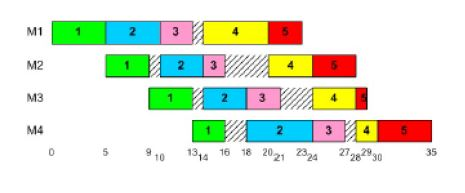
\includegraphics[scale=0.8]{IlusFlowShop}  
	\caption[Ilustrasi Flow Shop]{Ilustrasi Flow Shop} 
	\label{fig:IlusFlowShop} 
\end{figure}

Gambar ~\ref{fig:IlusFlowShop} merupakan ilustrasi proses flowshop scheduling. Pada gambar tersebut urutan pengerjaan
job adalah 1,2,3,4, dan 5. Masing-masing job memiliki 4 proses operasi dan masing-masing
proses operasi tersebut dikerjakan oleh mesin yang berbeda. Saat proses operasi 1 dari job 1 telah
selesai, mesin 2 akan mengerjakan proses operasi 2 dari job 1, dan mesin 1 akan mengerjakan proses
operasi 1 dari job 2.
Saat proses operasi 2 dari job 1 sudah selesai, mesin 2 akan mengerjakan proses operasi 3 dari
job 1, akan tetapi mesin 2 yang seharusnya mengerjakan proses operasi 2 dari job 2 akan mengalami
idle, karena proses operasi 1 dari job 2 belum selesai dikerjakan di mesin 1. 

Idle adalah kondisi dimana mesin tidak melakukan proses operasi apapun, baik itu karena adanya proses operasi yang
akan dilakukan pada mesin tersebut belum selesai diproses di mesin selanjutnya atau karena masih
ada proses operasi yang dilakukan pada mesin selanjutnya. 
Idle akan mempengaruhi besar kecilnya nilai makespan yang akan dihasilkan. Semakin banyak idle, maka makespan umumnya
akan semakin besar, serta sebaliknya dimana semakin sedikit idle maka umumnya makespan yang
didapat akan semakin kecil.
Mesin juga mengalami idle pada saat mesin 1 telah menyelesaikan proses operasi job 3 namun
ternyata pada mesin 2 proses job 2 belum selesai. Sehingga job 3 akan disimpan dalam mesin 1
hingga mesin 2 selesai mengerjakan proses operasi job 2.

\subsection{Karakteristik Penjadwalan Flow Shop}
\begin{enumerate}
	\item Terdapat n job yang tersedia dan siap diproses pada waktu t = 0.
	\item Waktu proses tiap job tidak bergantung pada urutan pengerjaan.
	\item Terdapat m mesin berbeda, yang tersedia secara kontinu.
	\item Operasi-operasi individual job pada tiap mesin tidak dapat dipecah-pecah.
\end{enumerate}

\section{Multi Objective Flow Shop Scheduling}
Pada dasarnya MOFSP adalah bagian dari {\it flow shop } itu sendiri. MOFSP menjelaskan kriteria optimasi yang akan diselesaikan menggunakan algoritma {\it Ant Colony Optimization}. Kriteria tersebut bersifat jamak {\it Multi Objective}. Kriteria tersebut misalnya saja minimasi waktu proses keseluruhan, minimasi waktu tunggu job, minimasi waktu nganggur mesin, dan sebagainya. Kriteria optimasi yang akan diselesaikan pada skripsi ini adalah menentukan makespan minimum dan minimasi waktu {\it idle} atau {\it tardiness}.

\section{Ant Colony Optimization}
Any Colony Optimization (ACO) awalnya dikembangkan oleh Marco Dorigo et. al. (1996). Algoritma ini didasarkan pada cara kerja semut untuk menentukan jarak terpendek dari sarang menuju sumber makanan. Semut dapat menemukan jarak terpendek dengan memanfaatkan jejak pheromone (air liur semut) yang dimanfaatkan sebagai komunikasi tidak langsung antar semut. Ketika semut berjalan, ia meninggalkan pheromone dalam jumlah tertentu pada jalur yang dilewatinya. Semut dapat mencium pheromone dan ketika memilih jalur mereka cenderung untuk memilih jalur dengan konsentrasi pheromone yang lebih besar adalah jarak terpendek.

Saat seekor semut yang terisolasi bergerak secara acak, semut ini akan mengikuti jejak yang telah ditinggalkan sebelumnya yang dapat dideteksi dan mempunyai tingkat probabilitas yang tinggi untuk diikuti dan melanjutkan jejak sebelumnya dengan pheromone baru. Tingkah laku kolektif yang muncul disebut dengan tingkah laku Autocalystic, dimana semut yang lain dapat mengikuti jejak yang ada dan jejak yang semakin jelas akan memudahkan bagi semut yang lain untuk mengikutinya. Proses ini secara khusus terjadi melalui kumpulan umpan balik yang positif, dimana kemungkinan semut untuk memilih pola meningkat seiring dengan jumlah semut yang sebelumnya mengikuti pola yang sama.
\begin{figure}[H]
	\centering
	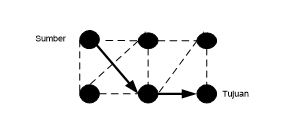
\includegraphics[scale=0.85]{gambar2}
	\caption[Jalur Solusi Semut] {Jalur Solusi Semut Ant Colony Optimization}
	\label{fig:JaluSolusiSemut}
\end{figure}
Marco Dorigo et. al. (1996) mengatakan bahwa Ant Colony Optimization adalah algoritma heuristik yang serba guna untuk memecahkan berbagai masalah optimasi. Algoritma ACO memiliki karakteristik sebagai berikut :
\begin{enumerate}
	\item Serba guna (versatile), dapat dipakai untuk memecahkan masalah dengan versi yang sama, seperti TSP dan Asymetric Travelling Salesman Problem (ATSP).
	\item Sempurna (robust), dapat diterapkan untuk memecahkan dengan hanya perubahan sedikit terhadap masalah optimasi yang lain, seperti Quadratic Assigment Problem dan Job shop Scheduling Problem (JSP).
	\item Pendekatan yang berbasis populasi.
\end{enumerate}

\subsection{Algoritma Ant Colony Optimization pada penjadwalan Flow Shop}
\begin{itemize}
\item Karakteristik Semut \\
	Sesuai dengan contoh pada gambar ~\ref{fig:karakteristiksemut1} terdapat pola saat sekelompok semut berjalan (contoh, dari sumber makanan A ke sarang E, dan sebaliknya). Secara tiba-tiba rintangan muncul dan pola menjadi terpotong. Pada posisi B, semut berjalan dari A ke E (atau pada posisi D yang bergerak dengan arah yang berlawanan) harus memutuskan apakah harus bergerak ke kiri atau ke kanan.
	Pilihan ini dipengaruhi oleh intensitas jejak pheromone yang ditinggalkan oleh semut sebelumnya. Tingkat pheromone yang lebih tinggi pada pola sebelah kanan memberikan semut rangsangan yang lebih kuat dan kemungkinan yang lebih tinggi untuk berbelok ke kanan. Semut pertama mencapai titik B atau D mempunyai kemungkinan yang sama untuk belok ke kiri atau ke kanan (karena tidak terdapat pheromone pada dua pola alternatif tersebut).
	
	Karena pola BCD lebih pendek dibandingkan dengan pola BHD, semut pertama yang mengikuti ini akan mencapai D sebelum semut yang mengikuti pola BHD. Hasilnya adalah semut yang bergerak dari E ke D akan mendapatkan jejak yang lebih jelas pada pola DCB, karena setengah dari semut tersebut yang memilih untuk mendekati rintangan melalui DCBA dan dengan segera akan sampai melalui BCD, mereka akan melalui pola memilih pola DCB dibandingkan pola DHB. 

	Sebagai Konsekuensi, jumlah semut yang mengikuti pola BCD per unit waktu akan lebih banyak dibandingkan dengan jumlah semut yang mengikuti pola BHD.
	Hal ini menyebabkan jumlah pheromone pada pola yang lebih pendek akan muncul lebih cepat dibandingkan dengan pola yang lebih jauh, dan oleh karena itu kemungkinan semut yang memilih pola yang diikuti mempunyai bias terhadap pola yang lebih pendek. Hasil akhir yang akan dipilih secara cepat akan ditunjukkan pada pola yang lebih pendek.	
	Algoritma yang akan dibahas pada bagian selanjutnya adalah model yang berasal dari kumpulan kehidupan nyata semut. Selanjutnya hal ini disebut dengan Sistem Semut dan algoritma yang akan dibahas dikenal dengan algoritma semut. Karakteristik semut asli untuk ketika sedang bergerak dari satu titik ke titik tujuan dapat dilihat pada kedua ilustrasi gambar berikut ini.
	
	\begin{figure}[H]
	\centering
	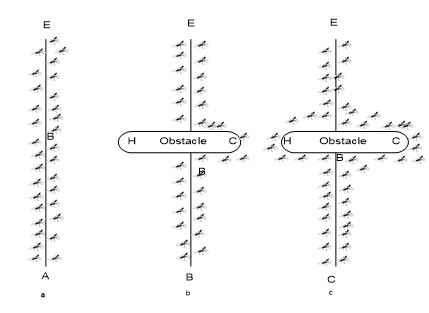
\includegraphics[scale=0.90]{gambar3}
	\caption[Contoh Karakteristik Semut] {Karakteristik semut}
	\label{fig:karakteristiksemut1}
	\end{figure}

Penjelasan karakteristik semut :
\begin{enumerate}
	\item Semut-semut mengikuti jalur dari titik A ke titik E.
	\item Sebagai rintangan maka diletakkan hambatan pada jalur lintasan ; semut-semut memilih untuk bergerak memutari salah satu sisi dengan probabilitas yang sama.
	\item Di jalur yang lebih pendek ditinggalkan lebih banyak pheromone.\\	
\end{enumerate}

\item Cara Kerja Algoritma
Berikut adalah flow chart dari algoritma ant colony.
\begin{figure}[H]
	\centering
	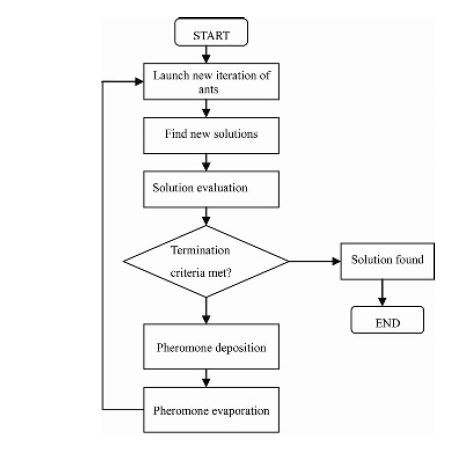
\includegraphics[scale=0.80]{gambar5}
	\caption[Flowchart ACO] {Flowchart algoritma ant colony optimization}
	\label{fig:flowchartACO}
\end{figure}
Berdasarkan flowchart ~\ref{fig:flowchartACO}, dalam menjalankan proses pelatihan dengan algoritma ant colony maka perlu diperrsiapkan
jalur-jalur yang ada perlu. Jalur-jalur tersebut merupakan kemungkinan
solusi-solusi yang mungkin dipilih oleh semut. Kemungkinan dipilihnya suatu jalur akan ditentukan berdasarkan nilai feromon, oleh karena itu perlu dibentuk pula tempat penyimpanan feromon untuk setiap jalur yang mungkin dilalui.

Pada awalnya, algoritma ant colony akan membentuk sekumpulan semut, semut-semut tersebut akan disebar secara acak pada jalur-jalur yang ada. Proses penyebaran semut tersebut akan memperhatikan nilai feromon dari masing-masing jalur. Semakin besar nilai feromon dari suatu jalur, maka semakin besar pula kemungkinan dipilihnya jalur tersebut untuk dilalui semut. Jalur-jalur yang dipilih oleh semut akan disimpan dan dibandingkan dengan jalur-jalur yang telah dipilih oleh semut-semut lainnya.

Dari jalur-jalur yang telah dipilih akan dibentuk nilai feromonnya berdasarkan tingkat keoptimalan
dari jalur tersebut. Nilai feromon-feromon tersebut akan ditambahkan pada jalur-jalur yang bersangkutan untuk memperbesar kemungkinan dipilihnya jalur tersebut sesuai dengan tingkat keoptimalannya. Semakin optimal suatu jalur, semakin besar pula jumlah feromon yang akan ditambahkan pada suatu jalur. Tidak lupa pula, proses evaporasi feromon akan dilakukan. Proses evaporasi feromon ini akan mengurangi jumlah feromon yang disimpan. Proses evaporasi ini bertujuan untuk mengurangi jumlah feromon dari jalur-jalur yang dianggap kurang optimal. Proses-proses tersebut akan terus
dilakukan hingga suatu kondisi berhenti ditemui.

\begin{figure}[H]
	\centering
	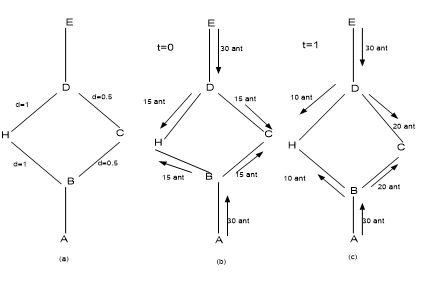
\includegraphics[scale=0.80]{gambar6}
	\caption[Pseudocode ACO] {Pseudocode algoritma ant colony optimization}
	\label{fig:pseudocodeACO}
\end{figure}

Dari flow chart ~\ref{fig:flowchartACO}, dibentuklah pseudocode di atas. Baris pertama
dari pseudocode tersebut merupakan proses pembentukan data feromon. Proses pembentukan data
feromon tersebut akan memperhatikan kasus yang ingin dicari hasil optimalnya. Nilai masingmasing
jalur dan cara mengartikan nilai feromon tersebut diatur berdasarkan kasus yang ingin
dicari hasil optimalnya. Jumlah feromon pada masing-masing jalur pada awalnya bernilai sama.
Setelah data feromon selesai dibuat, proses pelatihan dengan menggunakan algoritma ant colony
dimulai. Baris ketiga pada pseudocode menunjukkan kondisi berhenti untuk proses optimisasi dari
algoritma ant colony. 

Seluruh potongan kode di dalam kondisi while tersebut merupakan satu fase
pelatihan dari algoritma ant colony. Fase pelatihan tersebut terdiri dari proses pembentukan jalur,
penentuan solusi optimal, dan perubahan nilai feromon (penambahan dan evaporasi feromon).
Fase pelatihan dari algoritma ant colony bertujuan untuk membentuk data feromon yang mampu
menghasilkan solusi yang paling optimal. Pada setiap fase pelatihan ini akan dibentuk sejumlah
semut yang bertugas untuk menyimpan solusi acak/solusi lokal yang telah dipilih pada suatu fase
pelatihan. Semut-semut ini akan dianggap memilih sebuah jalur/solusi secara acak berdasarkan
nilai yang disimpan pada data feromon. Jika solusi acak tersebut lebih baik dari solusi optimal
yang diketahui pada saat ini, maka solusi acak tersebut akan dianggap sebagai solusi optimal yang
baru.

Pada saat pemilihan solusi secara acak, perlu dipastikan bahwa solusi tersebut merupakan solusi
yang valid dari suatu kasus. Pada saat pemilihan solusi kita juga dapat melakukan proses local
search. Proses ini bertugas untuk membandingkan solusi yang dibentuk dengan solusi yang mirip.
Jika solusi lain tersebut lebih baik, maka solusi yang dipilih akan diganti menjadi solusi yang mirip
tersebut. Proses ini bersifat opsional, karena tidak semua permasalahan dapat diaplikasikan dengan
proses ini.

Setelah semut-semut telah selesai memilih solusi secara acak, proses perubahan nilai feromon
akan dilakukan. Proses perubahan tersebut mencakup proses penambahan dan evaporasi nilai
feromon. Proses penambahan nilai feromon akan memperhatikan tingkat keoptimalan dari solusi
yang dipilih suatu semut. Semakin optimal suatu solusi, semakin banyak pula nilai feromon yang
ditambahkan pada jalur/solusi tersebut. Setelah proses optimisasi selesai, solusi yang paling optimal
akan diberikan sebagai data keluaran.

\end{itemize}

\section{Tailard Benchmark}
Dalam melakukan pengujian tingkat keoptimalan dari suatu algoritma, pengujian sebaiknya dilakukan dengan menggunakan data kasus standar. Data kasus standar tersebut akan dianggap sebagai suatu kasus unik yang memerlukan algoritma khusus untuk proses optimisasinya. Data standar tersebut akan digunakan sebagai pembanding dalam proses optimisasi. 
Dengan menggunakan data	standar, penilaian kualitas dari suatu algoritma optimisasi dapat dilakukan. Dalam kasus penelitian ini, data kasus standar tersebut akan menggunakan data dari suatu benchmark yang bernama {\it Taillard Benchmark}. {\it Benchmark} tersebut dapat diakses lewat url berikut : \footnote{\label{Tailard}\url{http://mistic.heig-vd.ch/taillard/problemes.dir/ordonnancement.dir/ordonnancement.html} } .

Taillard benchmark adalah sebuah web hosting yang menyediakan kumpulan data yang digunakan sebagai input dan akan menghasilkan output suatu permasalahan flow shop scheduling. Input dan output tersebut digunakan sebagai standar dalam pengujian algoritma penyelesaian flow shop
scheduling sesuai dengan yang didefinisikan oleh Taillard [9]. Hal ini akan mempengaruhi penilaian suatu algoritma dalam menyelesaikan permasalahan flow shop scheduling apakah algoritma tersebut sudah efektif atau tidak.

Dalam data input yang digunakan pada permasalahan flow shop scheduling, selain banyaknya job dan mesin, ada pula initial seed yang dapat digunakan menggunakan random generator. Initial Seed ini berfungsi dalam membuat variasi waktu proses dari tiap job yang ada, sehingga kumpulan
job yang ada akan memiliki waktu proses yang berbeda pada tiap prosesnya. Seperti yang telah diketahui sebelumnya, tujuan utama dari pencarian solusi permasalahan flow shop scheduling adalah pencarian waktu makespan yang paling kecil. Taillard benchmark Framework
ini akan menyediakan data output yang berupa upper bound dan lower bound solusi permasalah
flow shop scheduling. Lower bound menunjukkan batas makespan paling minimum sedangkan Upper bound menunjukkan batas makespan paling maksimum. Selain itu, Taillard benchmark juga akan memberikan data-data detail dari proses-proses yang dilakukan.Tampilan dari Tailard benchmark sebagai berikut :

\begin{figure}[H]
	\centering
	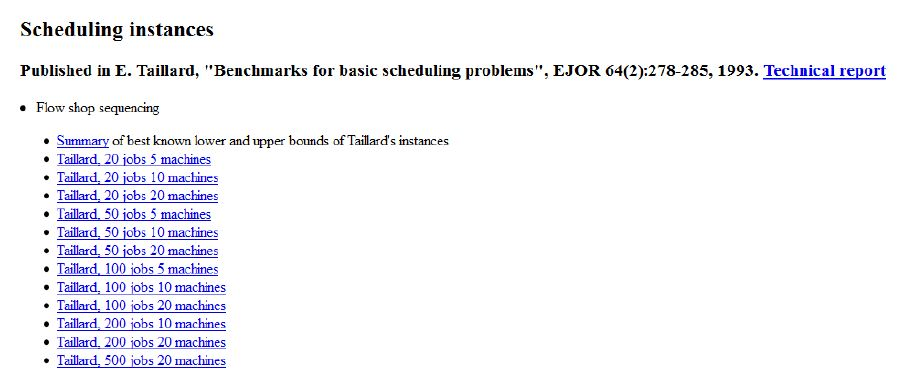
\includegraphics[scale=0.70]{tailard}
	\caption[Tailard Benchmark] {Tailard Benchmark}
	\label{fig:tailard1}
\end{figure}
Gambar ~\ref{fig:tailard1} memperlihatkan tampilan menu Taillard benchmark yang dimana kita dapat memilih
kasus-kasus flow shop scheduling yang hendak digunakan. Pada setiap kasusnya, telah disediakan
data-data input berupa jumlah job dan jumlah mesin dan initial seed. Selain itu diberikan
pula upper bound dan lower bound dari kasus tersebut untuk menjadi tolak ukur algoritma yang
telah kita buat apakah dapat memenuhi standar dari Taillard Benchmark.
Taillard membagi jenis kasus-kasus flow shop scheduling berdasarkan jumlah job dan jumlah
mesin. Pada tiap jenis kasus Taillard menyediakan 10 (sepuluh) kasus yang dapat dicoba.
\begin{figure}[H]
	\centering
	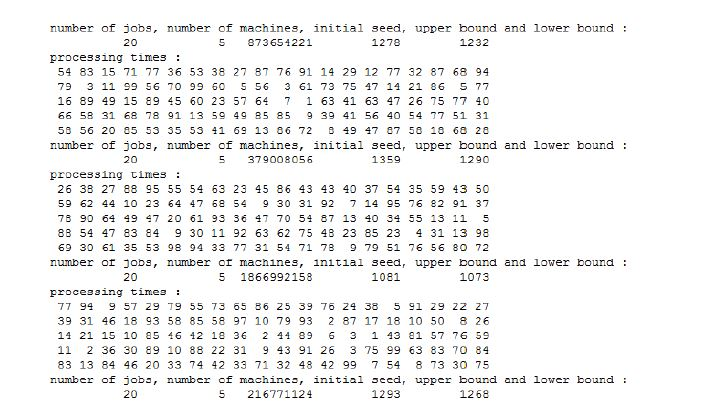
\includegraphics[scale=0.80]{tailard2}
	\caption[Contoh kasus Tailard Benchmark] {Contoh kasus Tailard Benchmark}
	\label{fig:tailard2}
\end{figure}
Gambar ~\ref{fig:tailard2} memperlihatkan tampilan salah satu kasus pada flow shop scheduling dengan 20
jobs dan 5 mesin. Pada gambar tersebut kita dapat melihat data waktu proses tiap job pada
tiap mesin. Waktu proses ini didapatkan seluruhnya berdasarkan initial seed yang digunakan.
Berdasarkan data tersebut, algoritma yang telah dibuat sebelumnya dapat dinilai apakah telah 
efektif atau belum sesuai dengan upper bound dan lower bound yang diberikan.











